% !TEX TS-program = pdflatex
% !TEX encoding = UTF-8 Unicode

% This is a simple template for a LaTeX document using the "article" class.
% See "book", "report", "letter" for other types of document.

\documentclass[11pt]{article} % use larger type; default would be 10pt

\usepackage[utf8]{inputenc} % set input encoding (not needed with XeLaTeX)

%%% Examples of Article customizations
% These packages are optional, depending whether you want the features they provide.
% See the LaTeX Companion or other references for full information.

%%% PAGE DIMENSIONS
\usepackage{geometry} % to change the page dimensions
\geometry{a4paper} % or letterpaper (US) or a5paper or....
% \geometry{margin=2in} % for example, change the margins to 2 inches all round
% \geometry{landscape} % set up the page for landscape
%   read geometry.pdf for detailed page layout information

\usepackage{graphicx} % support the \includegraphics command and options

% \usepackage[parfill]{parskip} % Activate to begin paragraphs with an empty line rather than an indent

%%% PACKAGES
\usepackage{booktabs} % for much better looking tables
\usepackage{array} % for better arrays (eg matrices) in maths
\usepackage{paralist} % very flexible & customisable lists (eg. enumerate/itemize, etc.)
\usepackage{verbatim} % adds environment for commenting out blocks of text & for better verbatim
\usepackage{subfig} % make it possible to include more than one captioned figure/table in a single float
% These packages are all incorporated in the memoir class to one degree or another...

%%% HEADERS & FOOTERS
\usepackage{fancyhdr} % This should be set AFTER setting up the page geometry
\pagestyle{fancy} % options: empty , plain , fancy
\renewcommand{\headrulewidth}{0pt} % customise the layout...
\lhead{}\chead{}\rhead{}
\lfoot{}\cfoot{\thepage}\rfoot{}

%%% SECTION TITLE APPEARANCE
\usepackage{sectsty}
\allsectionsfont{\sffamily\mdseries\upshape} % (See the fntguide.pdf for font help)
% (This matches ConTeXt defaults)

%%% ToC (table of contents) APPEARANCE
\usepackage[nottoc,notlof,notlot]{tocbibind} % Put the bibliography in the ToC
\usepackage[titles,subfigure]{tocloft} % Alter the style of the Table of Contents
\renewcommand{\cftsecfont}{\rmfamily\mdseries\upshape}
\renewcommand{\cftsecpagefont}{\rmfamily\mdseries\upshape} % No bold!

%%% END Article customizations

%%% The "real" document content comes below...

\title{STU33009 Mid-Term Assignment}
\author{Efeosa Louis Eguavoen - 17324649}
%\date{} % Activate to display a given date or no date (if empty),
         % otherwise the current date is printed 

\begin{document}
\maketitle
\newpage
\section{Question 1}
(a)
\begin{center}
	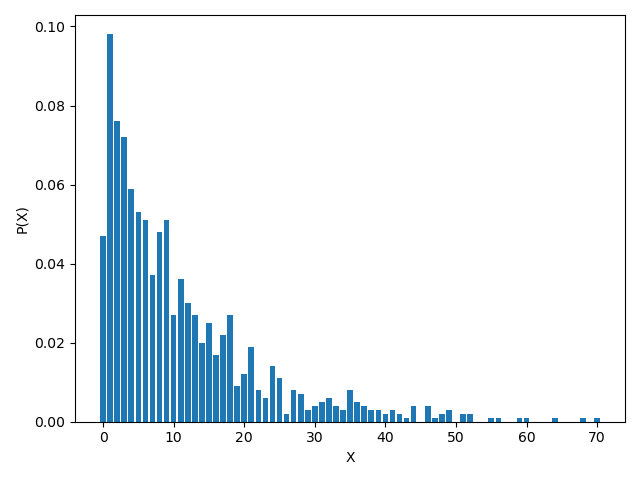
\includegraphics[scale=0.5]{hist1.png}
\end{center}
(b)
\newline 
To obtain this result I converted the times to dummy variables and set the sum of 1's over the total amount equal to the probability.
\[P(X_0 =1) = 0.38100 \]
(c)
\newline
One of the useful features of python is it calculates the standard deviation and mean for us alowing us just to plug in values for doing confidence intervals
To calculate it normally we'd use
\((1-P)(0-P)^2 + (P)(1-P)^2\) where \(P = P(X_0 =1) \)
We get \[\sigma^2 = 0.235839\]
To get the 95 percent interval for each method we get: where mean is = 0.381 and N = 1000
\newline
Chebyshevs: Provides an actual bound for all values of N but is loose in general.
\[.381 \pm \frac{\sqrt{.235839}}{\sqrt{.05(1000)}}\]
which equals
\[.381 \pm 0.06867\]
CLT: Full distribution of X hat but accuracy depends on size of N
\[-2(.485633) \leq X - 0.381 \leq  + 2(.485633)\]
\[-.972 \leq X- 0.381 \leq +.972\]
\section{Question 2}
Same method as Q1(b)
\[P(X_1 = 1) = 0.574\]
\[P(X_2 = 1) = 0.523\]
\[P(X_3 = 1) = 0.561\]
\section{Question 3}
Using the calculated \(P(X_i = 1)\) and the given \(P(U_n = i)\) we can calculate \(P(Z_n >10)\) using marginalisation by doing the following:
\[P(Z_n >10) = P(X_0 = 1)P(U_n = 0) + P(X_1 = 1)P(U_n=1) + ....+P(X_3 = 1)P(U_n=3)\]
giving us \(P(Z_n >10) = 0.5066 \)

\section{Question 4}
\[P(U_n = 0 | Z_n >10) = \frac{P(Z_n>10|U_n = 0)P(Z_n>10)}{P(U_n=0)}\]
\(P(Z_n>10|U_n = 0)\) is the probability of user 0 sending a bad signal which is the same as \( P(X_0 = 1)\)
Answer:
\[P(U_n = 0 | Z_n >10) = \frac{.381*0.5066}{0.27616531089096} = 0.6989\] 
\section{Question 5}
For this question, I generated a list of 1000 requests from a user i picked at random given the probabilities in the data given. Given the user a 0 or 1 is added to the list of requests based of \(P(X_i = 1) \). I then calculated  \(P(Z_n>10)\) by counting the number of 1's in the list and putting it over 1000(the number of requests).I then ran this 1000 times also to get the average value of \( Z_n >10\) This gave me:
\[P(Z_n>10) = 0.5071\]
Compared to Zn we calculated earlier, our stochastic simulation gives us a value very close to what we had estimated initially. The more times we run the simulation, we can see our accuracy improving over time due to the law of large numbers. Our answer is just an approximation of what Zn should be given N trials though leading to the different values.

\section{Code}
\begin{verbatim}
def graphMaker():
    dataFile = open("statsData", "r")
    user0Vals = []
    user1vals = []
    user2vals = []
    user3vals = []
    firstLine = True;
    for i in dataFile:
        if (not firstLine):
            vals = i.split(" ")
            user0Vals.append(int(vals[0]))
            user1vals.append(int(vals[1]))
            user2vals.append(int(vals[2]))
            user3vals.append(int(vals[3]))
        firstLine = False
    user_0 = 0.27616531089096
    user_1 = 0.21892050946049
    user_2 = 0.19773040565225
    user_3 = 0.3071837739963

    df = pd.DataFrame.from_records([user0Vals, user1vals, user2vals, user3vals])
    df = df.transpose()
    data = pd.DataFrame(df[0].value_counts())
    data.columns = ["Counts"]
    data["Prob"] = data["Counts"] / 1000

    df['Indicator1'] = 0
    df['Indicator2'] = 0
    df['Indicator3'] = 0
    df['Indicator4'] = 0

    df.loc[df[0] > 10, 'Indicator1'] = 1
    df.loc[df[1] > 10, 'Indicator2'] = 1
    df.loc[df[2] > 10, 'Indicator3'] = 1
    df.loc[df[3] > 10, 'Indicator4'] = 1

   # pmf = plt.bar(data.index.values, data["Prob"])
   # plt.xlabel("X")
   # plt.ylabel("P(X)")
  #  plt.show()
    u0_stats = df['Indicator1'].agg(['mean', 'std'])
    u1_stats = df['Indicator2'].agg(['mean', 'std'])
    u2_stats = df['Indicator3'].agg(['mean', 'std'])
    u3_stats = df['Indicator4'].agg(['mean', 'std'])

    p_Zn = (u0_stats['mean'] * user_0) + (u1_stats['mean'] * user_1) + (u2_stats['mean'] * user_2) \
           + (u3_stats['mean'] * user_3)  # current guess how to solve it
    print((p_Zn))
    print(u0_stats,'\n',u1_stats,'\n',u2_stats,'\n',u3_stats)
    return([u0_stats['mean'],u1_stats['mean'],u2_stats['mean'],u3_stats['mean']])


def stochastic_sim(means):
    order = np.random.choice(['user0','user1','user2','user3'],10000,
                     p=[0.27616531089096,0.21892050946049,
                        0.19773040565225,0.3071837739963])
    Zlist = []
    znList = []
    for s in range(1000):
        for i in order:
            if i == 'user0':
                Zlist.append(np.random.choice([0, 1], 1, p=[1 - means[0], means[0]])[0])
            elif i == 'user1':
                Zlist.append(np.random.choice([0, 1], 1, p=[1 - means[1], means[1]])[0])
            elif i == 'user2':
                Zlist.append(np.random.choice([0, 1], 1, p=[1 - means[2], means[2]])[0])
            elif i == 'user3':
                Zlist.append(np.random.choice([0, 1], 1, p=[1 - means[3], means[3]])[0])
        zFrame = pd.DataFrame(Zlist)
        znList.append(zFrame[0].agg(['mean']))
        Zlist = []
        print(s)
    print(sum(znList)/1000)
means = graphMaker()
stochastic_sim(means)
\end{verbatim}
\end{document}
